%Sistemas a eventos discretos

\chapter{Fundamenta\c{c}\~ao Te\'orica}

Neste cap\'itulo ser\'a apresentado uma fundamenta\c{c}\~ao te\'orica sobre sistemas a eventos discretos.

\section{Sistemas a eventos discretos}

%introducao: falar o que e e como pode ser modelado
Segundo \cite{apostilacury}, sistemas a eventos discretos s\~ao sistemas que percebem as ocorr\^encias no ambiente \`a sua volta, denominados eventos. Percep\c{c}\~ao de uma mudan\c{c}a de estado em um sensor e o in\'icio e t\'ermino de uma tarefa s\~ao exemplos de eventos instant\^aneos, o que lhes confere um car\'ater discreto no tempo. A natureza discreta do evento faz com que esses sistemas sejam modelos pr\'aticos de sistemas complexos, podendo representar a l\'ogica e o dinamismo de um sistema \cite{moody1998}.

V\'arios tipos de modelagem para SEDs foram desenvolvidos. Os modelos que mais tem dado forte contribui\c{c}\~oes ao desenvolvimento da teoria de controle de SEDs s\~ao: Ramadge-Wonham baseado na teoria de aut\^omatos e Redes de Petri \cite{apostilacury}.


%Tais sistemas est ̃ao presentes em uma s ́erie de aplica ̧c ̃oes, incluindo por exemplo aautoma ̧c ̃ao da manufatura, a rob ́otica, a supervis ̃ao de tr ́afego, a log ́ıstica (canaliza ̧c ̃ao earmazenamento de produtos, organiza ̧c ̃ao e presta ̧c ̃ao de servi ̧cos), sistemas operacionais,redes de comunica ̧c ̃ao de computadores, concep ̧c ̃ao de software, gerenciamento de basesde dados e otimiza ̧c ̃ao de processos distribu ́ıdos. Tais sistemas tˆem em comum a maneirapela qual percebem as ocorrˆencias no ambiente `a sua volta, o que se d ́a pela recep ̧c ̃ao deest ́ımulos, denominados eventos. S ̃ao exemplos de eventos o in ́ıcio e o t ́ermino de umatarefa e a percep ̧c ̃ao de uma mudan ̧ca de estado em um sensor. Estes eventos s ̃ao, por suanatureza, instantˆaneos, o que lhes confere um car ́ater discreto no tempo. Sistemas comestas caracter ́ısticas s ̃ao denominados sistemas a eventos discretos (SED), 


\section{Redes de Petri}
%Redes de Petri: criacao, estrutura, dinamica e propriedades

Desenvolvido por C. A. Petri no in\'icio dos anos 1960, Redes de Petri \'e um modelo de SEDs que possui algumas similariedades com os aut\^omatos, como a representa\c{c}\~ao atrav\'es de grafos e tamb\'em a manipula\c{c}\~ao de eventos de acordo com regras especificadas \cite{Cassandras2008}. A RdP \'e composta por transi\c{c}\~oes, lugares, marca\c{c}\~oes e arcos. As transi\c{c}\~oes est\~ao diretamente relacionada aos eventos, e s\~ao efetuadas caso seus pr\'e-requisitos estejam satisfeitos. Os lugares associado as suas marca\c{c}\~oes, atrav\'es de fichas, podem representar o estado da rede, e tamb\'em servem como condi\c{c}\~ao para o disparo de uma transic\c{c}\~ao. Os arcos ligam lugares a transi\c{c}\~oes e vice-versa, e podem possuir um peso que altera a quantidade de marca\c{c}\~oes para o disparo de uma transi\c{c}\~ao ou tamb\'em alterar a quantidade de marca\c{c}\~oes que um lugar recebe ap\'os o disparo de uma transi\c{c}\~ao.
O processo de modelagem da RdP se inicia com o desenho de sua estrutura composta pelo conjunto de elementos (P,T,A,$\omega$), onde P \'e o conjunto de lugares, T \'e o conjunto de transi\c{c}\~oes, A \'e o conjunto de arcos e $\omega$ o conjunto de pesos dos arcos. Na figura \ref{fig:rdpsimples} \'e apresentado uma RdP simples, definida por P=\{p\textsubscript{1},p\textsubscript{2}\}, T=\{t\textsubscript{1},t\textsubscript{2}\}, A=\{(p\textsubscript{1},t\textsubscript{1}),(t\textsubscript{1},p\textsubscript{2}),(p\textsubscript{2},t\textsubscript{2}),(t\textsubscript{2},p\textsubscript{1})\}, com  $\omega$(p\textsubscript{1},t\textsubscript{1})=1, $\omega$(t\textsubscript{1},p\textsubscript{2})=1, $\omega$(p\textsubscript{2},t\textsubscript{2})=1 e $\omega$(t\textsubscript{2},p\textsubscript{1})=1.

\begin{figure}[!htb]
	%\captionsetup{width=0.97\textwidth}
	\caption[Grafo de uma simples Rede de Petri]{Grafo de uma simples Rede de Petri.}
	\label{fig:rdpsimples}
	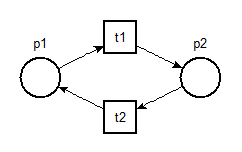
\includegraphics[width=6cm]{./figuras/RDP_SIMPLES.png}\centering
	\fonte{Autoria pr\'opria.}
\end{figure}


Ap\'os a modelagem de sua estrutura, o pr\'oximo passo \'e definir as marca\c{c}\~oes iniciais. O conjunto de marca\c{c}\~oes iniciais \'e definido por M\textsubscript{0}, denotada como M\textsubscript{0}=[M(p\textsubscript{1}),M(p\textsubscript{2}),...,M(p\textsubscript{n})], sendo M(p\textsubscript{n}) a quantidade de marca\c{c}\~oes, ou fichas, para o lugar p\textsubscript{n}.
Assim, para o exemplo da figura \ref{fig:rdpsimplesmarcada}, o conjunto das marca\c{c}\~oes iniciais \'e M\textsubscript{0} = [1,0].

\begin{figure}[!htb]
	%\captionsetup{width=0.97\textwidth}
	\caption[Grafo de uma simples Rede de Petri marcada]{Grafo de uma simples Rede de Petri marcada.}
	\label{fig:rdpsimplesmarcada}
	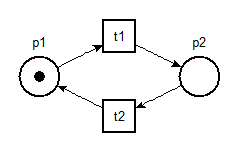
\includegraphics[width=6cm]{./figuras/RDP_SIMPLES_MARCADA.png}\centering
	\fonte{Autoria pr\'opria.}
\end{figure}

Assim obtemos o modelo completo da RdP, definida como uma qu\'intupla N = (P,T,A,$\omega$,M\textsubscript{0}).

O comportamento de uma RdP pode ser analisado atrav\'es de diversos m\'etodos. Entre as principais an\'alises est\~ao: limitabilidade, vivacidade e reversibilidade. Neste trabalho, destaca-se tamb\'em a an\'alis de invariantes de lugar.

\subsection{Limitabilidade}

Se o n\'umero de fichas cresce infinitamente em uma RdP, o sistema \'e considerado inst\'avel. Limitabilidade se refere a propriedade de um lugar manter um certo n\'umero de fichas. Uma RdP \'e k-limitada quando o n\'umero de fichas em cada lugar n\~ao exceda k em toda a sua evolu\c{c}\~ao.

\subsection{Vivacidade}

A RdP \'e dita viva quando sempre h\'a uma sequ\^encia de disparo que possa ser executada, ou seja, a RdP n\~ao ficar\'a impedida de evoluir por falta de transi\c{c}\~oes desabilitadas. A vivacidade representa a aus\^encia de "deadlocks", situa\c{c}\~ao em que a RdP fica presa. A RdP da Figura \ref{fig:rdpdeadlock} a RdP n\~ao \'e viva, pois o disparo de t\textsubscript{2} todas as fichas s\~ao consumidas.

\begin{figure}[!htb]
	%\captionsetup{width=0.97\textwidth}
	\caption[Rede de Petri com deadlock]{Rede de Petri com Deadlock.}
	\label{fig:rdpdeadlock}
	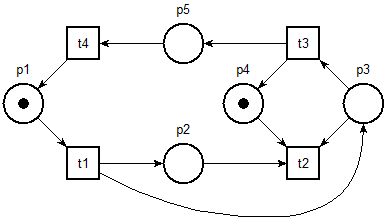
\includegraphics[width=6cm]{./figuras/RDP_DEADLOCK.png}\centering
	\fonte{Autoria pr\'opria.}
\end{figure}

\subsection{Reversibilidade}

A RdP \'e revers\'ivel se ap\'os uma sequ\^encia de disparos, \'e poss\'ivel voltar ao estado de marca\c{c}\~ao inicial M\textsubscript{0}.

\subsection{Invariantes de lugar}

Uma das propriedades estruturais de RdP que depende somente da topologia estrutural e n\~ao na marca\c{c}\~ao inicial da rede, \'e as invariantes de lugar \cite{moody1998}. As invariantes de lugar correspondem a um conjunto de lugares, nos quais, a contagem de ficha das marca\c{c}\~oes permanecem constantes.
%As invariantes de lugar ser\'a utilizado para identificar o rastro das fichas em uma RdP.



\section{Teoria de controle supervis\'orio}
Na d\'ecada de 80, P. J. Ramadge e W. M. Wonham desenvolveram um trabalho sobre controle de sistemas a eventos discretos que ficou conhecida como Teoria de Controle Supervis\'orio. Considere um cen\'ario que uma planta industrial necessita operar de forma ordenada e que a planta possui diversos sub-sistemas com comportamentos pr\'oprios, cada um formado por estados e conjuntos de eventos control\'aveis e n\~ao control\'aveis. As a\c{c}\~oes realizadas na planta, como o acionamento de uma esteira, s\~ao exemplos de eventos control\'aveis e as rea\c{c}\~oes dessas a\c{c}\~oes s\~ao eventos n\~ao control\'aveis, como o sinal de um sensor de presen\c{c}a. Segundo \cite{apostilacury}, para que os sub-sistemas atuem de forma coordenada, introduz-se um agente de controle denominado supervisor que deve observar os eventos ocorridos e difinir que evento, dentro do conjunto de eventos control\'aveis, ser\'a permitido que ocorra. O sistema \'e estruturado numa malha fechada, ilustrado na figura \ref{fig:tcsmalhafechada}.

\begin{figure}[!htb]
	%\captionsetup{width=0.97\textwidth}
	\caption[Sistema a evento discreto em malha fechada]{Sistema a evento discreto em malha fechada.}
	\label{fig:tcsmalhafechada}
	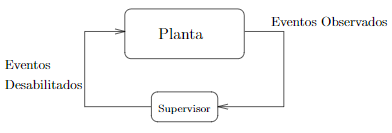
\includegraphics[width=6cm]{./figuras/TCS_EM_MALHA_FECHADA.png}\centering
	\fonte{\cite{apostilacury}}
\end{figure}

%The control problem will be considered fully solved when a controller that forces the specification to be met has been shown to exist and to be construcible. In accordance with widely accepted control methodology, we take the state desciption of a system (and, in this case, a language) to be fundamental.


\subsection{S\'intese de supervisores \'otimos}
A s\'intese de um supervisor \'otimo se baseia em tr\^es passos; obten\c{c}\~ao de um modelo para a planta a ser controlada, obten\c{c}\~ao de um modelo de representa\c{c}\~ao das especifica\c{c}\~oes a serem respeitadas e o terceiro passo \'e a s\'intese de uma l\'ogica de controle n\~ao bloqueante e \'otima \cite{apostilacury}.

A obten\c{c}\~ao do modelo da planta pode ser realizada atrav\'es do produto s\'incrono das modelagens de seus sub-sistemas. O produto s\'incrono \'e uma maneira de combinar diversos SEDs em um apenas um modelo. A especifica\c{c}\~ao \'e um modelo que ir\'a ditar o comportamento da planta, seu modelo tamb\'em pode ser representado atrav\'es de aut\^omatos e deve conter os eventos n\~ao control\'aveis e seus precedentes ou sucedentes control\'aveis de interesse. 
O c\'alculo para se encontrar o supervisor \'otimo baseia-se num procedimento iterativo que identifica maus estados no produto s\'incrono dos modelos da planta e da especifica\c{c}\~ao, isso resulta em um aut\^omato que dita quais eventos de controle pode ser realizado sobre a planta \cite{apostilacury}.
O problema de controle ser\'a solucionado quando um controlador que force a especifica\c{c}\~ao exista e seja contrut\'ivel \cite{WonhamCai2018}. Um exemplo pr\'atico do uso da Teoria de Controle Supervis\'orio ser\'a explorado no cap\'itulo 4 sobre a metodologia de acoplamento de supervisores \'otimos em RdP de Uzam e Wonham.

